%---------------------------------------------------------------------
% Course 	: Introduction To web sciences
% Professor : Dr.Nelson
% Name   	: Babitha Bokka
% Assignment: 3
%---------------------------------------------------------------------
\documentclass[12pt]{article}
%--------------------------------------------------------------------
% packages required
%--------------------------------------------------------------------
\usepackage{graphicx}
\usepackage{listings}
\usepackage{hyperref}
\usepackage{caption}
\usepackage{color}
\graphicspath{ {images/} }
%--------------------------------------------------------------------
% Start Margins
%--------------------------------------------------------------------
\addtolength{\oddsidemargin}{-.875in}
\addtolength{\evensidemargin}{-.875in}
\addtolength{\textwidth}{1.75in}
\addtolength{\topmargin}{-.885in}
\addtolength{\textheight}{1.95in}
%-------------------------------------------------------------------
% End Margins
%--------------------------------------------------------------------
\definecolor{codegreen}{rgb}{0,0.6,0}
\definecolor{codegray}{rgb}{0.5,0.5,0.5}
\definecolor{codepurple}{rgb}{0.58,0,0.82}
\definecolor{backcolour}{rgb}{0.95,0.95,0.92}

\lstdefinestyle{mystyle}{
    backgroundcolor=\color{backcolour},   
    commentstyle=\color{codegreen},
    keywordstyle=\color{magenta},
    numberstyle=\tiny\color{codegray},
    stringstyle=\color{codepurple},
    basicstyle=\footnotesize,
    breakatwhitespace=false,         
    breaklines=true,                 
    captionpos=b,                    
    keepspaces=true,                 
    numbers=left,                    
    numbersep=5pt,                  
    showspaces=false,                
    showstringspaces=false,
    showtabs=false,                  
    tabsize=2
}

\lstset{style=mystyle}


\begin{document}
%---------------------------------------------------------------------
%Making the title page
%---------------------------------------------------------------------
\begin{titlepage}
\title{INTRODUCTION TO WEB SCIENCES:\\*Assignment 3}
\author{Babitha Bokka}
\date{4 october 2014}
\maketitle
\end{titlepage}

%---------------------------------------------------------------------
%Table of contents
%---------------------------------------------------------------------
\tableofcontents
\newpage
%------------------------------------------------------------------
%Question 1
%------------------------------------------------------------------
\section{Question 1}
Download HTML content of 1000 URIs extracted in assignment 2.
%------------------------------------------------------------------
% approach
%------------------------------------------------------------------
\subsection{Approach Towards the Solution}
There are many good ways to extract the HTML from a URL. I approached the problem by using
\begin{enumerate}
	\item Requests
	\item urllib2 
	\item curl 
\end{enumerate}
\subsubsection{Desciption of extractHtml.sh}
\begin{enumerate}
	\item Open ,Read each line from uniqueUri.txt.
	\item Generate a md5 for each URI and store in a file.
	\item Using curl extract the HTML content .
\end{enumerate}
\subsubsection{Desciption of scrapeHtml.sh}
\begin{enumerate}
	\item Open a folder extract each file.
	\item Get the basename of the file.
	\item Using lynx get the data by stripping of the HTML.
	\item Store it in Plain file.
\end{enumerate}
\subsection{Observation}
Due to the different approaches to extract the HTML content an observation that curl extracts more HTML content that requests  and urllib2 library in python.So ,for this part of the assignment Shell script using curl is the best approach.
\newpage
%------------------------------------------------------------------
% Source Codes
%------------------------------------------------------------------
\subsection{Source Code to extract the HTML content}
\subsubsection{extractHtml.sh}
\lstinputlisting[breaklines=True,language=Python]{../Q1/extractHtml.sh}
\subsubsection{requestsExtractHtml.py}
\lstinputlisting[breaklines=True,language=Python]{../Q1/requestsExtractHtml.py}
\subsubsection{urllibExtractHtml.py}
\lstinputlisting[breaklines=True,language=Python]{../Q1/urllibExtractHtml.py}
\subsection{Source Code to strip the HTML from raw files}
\subsubsection{stripHtml.sh}
\lstinputlisting[breaklines=True,language=Python]{../Q1/stripHtml.sh}
\newpage
%------------------------------------------------------------------
% input file
%------------------------------------------------------------------
\subsection{InputFile : uniqueUri.txt}

The input is taken from the assignment 2 , the 1000 unique URIs.
\lstinputlisting[breaklines=True]{../Q1/urlFinalForDoc.txt}
\newpage
%------------------------------------------------------------------
% output files %------------------------------------------------------------------
\subsection{OutputFiles}
\subsubsection{md5Uri.txt}
A sample of URIs and their MD5 hash code.\\*
\lstinputlisting[breaklines=True]{../Q1/md5UriForDoc.txt}
\subsubsection{2c46a0201b5a19f93e19a0ace98cfb92.htm}
A sample of raw HTML file.\\*
\lstinputlisting[breaklines=True]{../Q1/rawhtmlForDoc.txt}
\newpage
\subsubsection{2c46a0201b5a19f93e19a0ace98cfb92.txt}
A sample of processed HTML file.\\*
\lstinputlisting[breaklines=True]{../Q1/plainhtmlForDoc.txt}
\subsection{Learnings}
\begin{enumerate}
	\item Shell script
	\item Python
\end{enumerate}
\subsection{Mistakes}
\begin{enumerate}
	\item For some reason ``lynx'' program was not extracting the data from the htm files instead it had an error message ``This site requires JavaScript and Cookies to be enabled. Please change your browser settings or upgrade your browser''. The files had this error message because in lynx program the path to the raw files if not specified so, that the lynx program would find them and strip out the html since there is no path the files had this error message.
	\item One should always check for ``CR'' and ``LF'' returns from windows to unix environment. 
\end{enumerate}
\subsection{Testing}
To test why the error message is stored in the plain files instead of actual data I loaded my raw file into my friend Mallika program then I realized the mistake and learnt why it happened.
\newpage

%------------------------------------------------------------------
%Question 2
%------------------------------------------------------------------
\section{Question 2}
Choose a keyword that matches atleast 10 documents .Count the occurrence of word and total number of words in each document and calculate the TF,IDF ,TF-IDF values.
\subsection{Approach Towards the Solution}
Keyword to searched in the extracted data is ``food'' . There are 835 total documents and 84 docs with the key word .This is when we assume that our the 1000 unique links are the total corpus.so,the IDF:\\*
 total docs in corpus = 835 \\*
 docs with term       = 84 \\*
lets assume the total corpus is 20B if bing has 20B documents indexed \\*
then \\*
 total docs in corpus = 20000000000 \\*
 docs with term       = 653000000 \\*
 
the TF values would be keyword count over total number of words.\\*

\subsubsection{Desciption of findKeyword.sh}
\begin{enumerate}
	\item Find a keyword and check the count in all the documents.
	\item Use  grep to count the keyword in all the processed files.
	\item save the count and file name .
\end{enumerate}

\subsubsection{Desciption of calculationProgram.py}
\begin{enumerate}
	\item Open ,read the file cal.txt
	\item File has key word count(k\_count),total count(t\_count),filename,URI.
	\item Store the (k\_count),(t\_count)and compute the TF,IDF,TFIDF.
	\item The results are stored in output1.txt and output2.txt.
\end{enumerate}
\newpage
%------------------------------------------------------------------
% Source Codes
%------------------------------------------------------------------
\subsection{Source Code}
\subsubsection{shellCommands.txt}
\lstinputlisting[breaklines=True,language=Python]{../Q2/shellCommands.txt}

\subsubsection{findKeyword.sh}
\lstinputlisting[breaklines=True,language=Python]{../Q2/findKeyword.sh}

\subsubsection{calculationProgram.py}
\lstinputlisting[breaklines=True,language=Python]{../Q2/calculationProgram.py}
\newpage
%------------------------------------------------------------------
% output files
%------------------------------------------------------------------
\subsection{Output Files}
\subsubsection{sort.txt}
\lstinputlisting[breaklines=True,language=Python]{../Q2/sortForDoc.txt}

\subsubsection{countData.txt}
\lstinputlisting[breaklines=True,language=Python]{../Q2/countData.txt}
\newpage
\subsubsection{Assuming the total docs in corpus is the total (835/1000) unique URIs we are dealing with and docs with term is the number of docs with the keyword(84/835)}
\lstinputlisting[breaklines=True,language=Python]{../Q2/output1.txt}

\subsubsection{Assuming the total docs in corpus is the total (20B)and docs with term is the number of docs with the keyword(65M)}
\lstinputlisting[breaklines=True,language=Python]{../Q2/output2.txt}
\newpage
\subsubsection{screenShot}
\begin{figure}[ht]
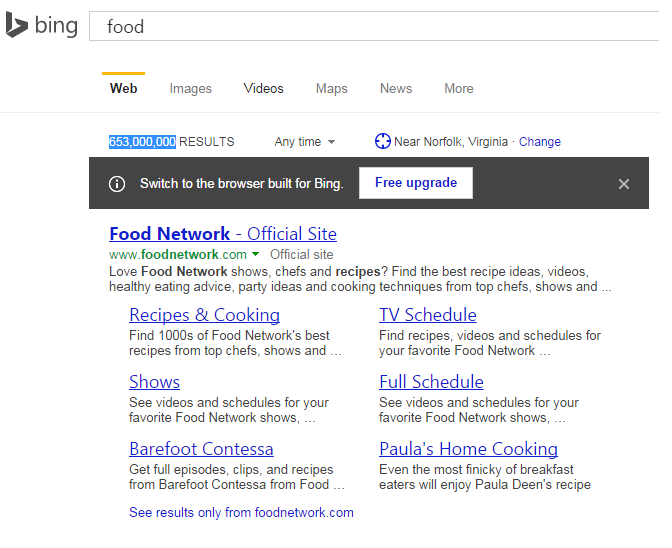
\includegraphics[scale=0.7]{../Q2/screenShot}
\centering
\caption{docs with term on web }
\end{figure}
\newpage

%------------------------------------------------------------------
% table for TF values
%------------------------------------------------------------------

\begin{center}
\begin{table}
\small
\begin{tabular}{ | p{3.0cm} | p{3.0cm} |p{3.0cm} | p{8.0cm} | }\hline
\textbf{TFIDF} & \textbf{TF} & \textbf{IDF} & \textbf{URI} \\\hline
0.159 & 0.048 & 3.313 & \url{http://ifoodi.blogspot.com } \\\hline
0.166 & 0.050 & 3.313 & \url{ http://turtlestravel.com} \\\hline
0.018 & 0.005 & 3.313 & \url{ http://howchow.blogspot.com} \\\hline
0.045 & 0.013 & 3.313 & \url{ http://thescienceofeating.com} \\\hline 
0.167 & 0.050 & 3.313 & \url{ http://www.cookinglight.com} \\\hline
0.289 & 0.087 & 3.313 & \url{http://foodnex.tumblr.com} \\\hline
0.010 & 0.003 & 3.313 & \url{ http://baconforthesoul.wordpress.com} \\\hline
0.023 & 0.007 & 3.313 & \url{ http://rockinrina.tumblr.com} \\\hline
0.038 & 0.011 & 3.313 & \url{ http://thedaintypig.com} \\\hline
0.013 & 0.004 & 3.313 & \url{ http://oxymoron101.wordpress.com} \\\hline
\end{tabular}
\caption{Total docs in corpus =835:docs with term = 84}
\end{table}
\end{center}


\begin{center}
\begin{table}
\small
\begin{tabular}{ | p{3.0cm} | p{3.0cm} |p{3.0cm} | p{8.0cm} | }\hline
\textbf{TFIDF} & \textbf{TF} & \textbf{IDF} & \textbf{URI} \\\hline
0.237 & 0.048 & 4.936 & \url{http://ifoodi.blogspot.com } \\\hline
0.248 & 0.050 & 4.936 & \url{ http://turtlestravel.com} \\\hline
0.028 & 0.005 & 4.936 & \url{ http://howchow.blogspot.com} \\\hline
0.067 & 0.013 & 4.936 & \url{ http://thescienceofeating.com} \\\hline 
0.248 & 0.050 & 4.936 & \url{ http://www.cookinglight.com} \\\hline
0.431 & 0.087 & 4.936 & \url{http://foodnex.tumblr.com} \\\hline
0.015 & 0.003 & 4.936 & \url{ http://baconforthesoul.wordpress.com} \\\hline
0.035 & 0.007 & 4.936 & \url{ http://rockinrina.tumblr.com} \\\hline
0.057 & 0.011 & 4.936 & \url{ http://thedaintypig.com} \\\hline
0.020 & 0.004 & 4.936 & \url{ http://oxymoron101.wordpress.com} \\\hline
\end{tabular}
\caption{Total docs in corpus = 20B:docs with term = 65M}
\end{table}
\end{center}
\newpage
%------------------------------------------------------------------
%Question 3
%------------------------------------------------------------------
\section{Question 3}
Get the page rank for 10 URIs from question 2.
\subsection{Approach Towards the Solution}
Go to the provided link and type the URL and solve the captcha to prove that you are human.\\*
The result will be the page rank to normalize it divide it by 10 or you can take the highest value and divide each page rank with the highest value .

\subsubsection{Desciption}
\begin{enumerate}
	\item Go to \url {http://www.prchecker.info/check_page_rank.php}.
	\item Solve the captcha.
	\item Write down the page rank given note that all pages on web are not ranked and the result of them will be not avialable.
\end{enumerate}

%------------------------------------------------------------------
% Source Codes
%------------------------------------------------------------------
\subsection{Source}
\subsubsection{sourceLink.txt}
\lstinputlisting[breaklines=True,language=Python]{../Q3/sourceLink.txt}

%------------------------------------------------------------------
% output files
%------------------------------------------------------------------
\subsection{Output Files}
\subsubsection{pageRank.txt}
\lstinputlisting[breaklines=True,language=Python]{../Q3/pageRank.txt}
\newpage
%------------------------------------------------------------------
% table for TF values
%------------------------------------------------------------------

\begin{center}
\begin{table}
\small
\begin{tabular}{ | p{4.0cm} | p{12.0cm} | }\hline
\textbf{Page Rank} & \textbf{URI} \\\hline
0   & \url{http://ifoodi.blogspot.com } \\\hline
0.3 & \url{ http://turtlestravel.com} \\\hline
0.4 & \url{ http://howchow.blogspot.com} \\\hline
0.2 & \url{ http://thescienceofeating.com} \\\hline 
0.7 & \url{ http://www.cookinglight.com} \\\hline
0.3 & \url{http://foodnex.tumblr.com} \\\hline
0   & \url{ http://baconforthesoul.wordpress.com} \\\hline
0   & \url{ http://rockinrina.tumblr.com} \\\hline
0.1 & \url{ http://thedaintypig.com} \\\hline
0.1 & \url{ http://oxymoron101.wordpress.com} \\\hline
\end{tabular}
\caption{Normalized page rank}
\end{table}
\end{center}

\subsection{Compare and Contrast rankings in Question 2 and Question 3}

When we compare the rankings based on TFIDF and page rank there is no relation between them.Rankings given by page rank and TFIDF have no corelation when you observe the page rank of \url {http://ifoodi.blogspot.com} and TFIDF value the page rank is 0 and TFIDF value is 0.237 . So, we cannot compare the values of page rank and TFIDF.


\newpage
%-------------------------------------------------------------------
%References
%-------------------------------------------------------------------
\bibliographystyle{plain}
\bibliography{A3_report}
\cite{*}
\end{document}






















